\chapter{LaTeX 排版功能演示}\label{ch:example}

\section{二级标题}
\subsection{三级标题}
\subsubsection{四级标题}
\paragraph{五级标题}
\subparagraph{六级标题}
正文内容

\section{列表展示：有序、无序与嵌套}

% 无序列表 (Unordered List)
\subsection{无序列表示例}
这是一段关于无序列表的介绍：
\begin{itemize}
  \item 第一项内容。
  \item 第二项内容，包含更多细节说明。
  \item 第三项内容。
\end{itemize}

% 有序列表 (Ordered List)
\subsection{有序列表示例}
以下是操作步骤：
\begin{enumerate}
  \item 第一步：准备原始数据。
  \item 第二步：编写 LaTeX 源码。
  \item 第三步：编译并检查 PDF 结果。
\end{enumerate}

% 嵌套列表 (Nested List)
\subsection{嵌套列表展示}
在复杂的文档逻辑中，我们经常需要嵌套使用列表：
\begin{enumerate}
  \item 第一阶段：文档规划
        \begin{itemize}
          \item 确定论点。
          \item 搜集参考文献。
        \end{itemize}
  \item 第二阶段：实际撰写
        \begin{itemize}
          \item 编写引言。
          \item 绘制图表。
                \begin{enumerate}
                  \item 数据清洗。
                  \item 绘图工具选择。
                \end{enumerate}
        \end{itemize}
\end{enumerate}

\section{数学公式排版}
\LaTeX{} 的核心优势在于其卓越的数学表达能力。根据排版位置的不同，数学模式主要分为两类：

\begin{equation}
  \int_{-\infty}^{\infty} e^{-x^2} \, dx = \sqrt{\pi}\label{eq:example_gauss}
\end{equation}

\subsection{多行对齐与连续等式}
对于推导过程，推荐使用 \texttt{amsmath} 宏包提供的 \texttt{aligned} 环境，利用 \texttt{\&} 符号对齐等号，实现整齐的推导链路：

\begin{equation}
  \begin{aligned}
    (a + b)^2 & = (a + b)(a + b)      \\
              & = a^2 + ab + ba + b^2 \\
              & = a^2 + 2ab + b^2
  \end{aligned}
\end{equation}

\subsection{矩阵与分段函数}
复杂的代数结构如矩阵，可以使用 \texttt{bmatrix}（带方括号）或 \texttt{pmatrix}（带圆括号）环境：

\begin{equation}
  \mathbf{A} =
  \begin{bmatrix}
    a_{11} & a_{12} \\
    a_{21} & a_{22}
  \end{bmatrix}, \quad
  \text{det}(\mathbf{A}) = a_{11}a_{22} - a_{12}a_{21}
\end{equation}

对于条件表达式或分段函数，则使用 \texttt{cases} 环境：

\begin{equation}
  f(n) =
  \begin{cases}
    n/2,  & \text{if } n\space\text{is even} \\
    3n+1, & \text{if } n\space\text{is odd}  \\
  \end{cases}
\end{equation}

\section{图像插入与浮动体}
借助 \texttt{graphicx} 宏包，可以精确控制图像的缩放与位置。除了基础的单图插入，\LaTeX{} 还支持并排显示和强制位置固定。
819
\subsection{基础单图}
最常见的插入方式，图片宽度通常设置为文本宽度的 60\% 到 80\%。

\begin{figure}[htbp]
  \centering
  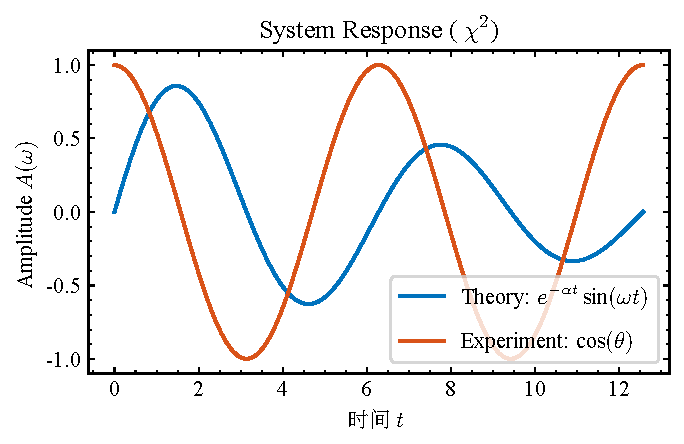
\includegraphics[width=0.6\textwidth]{figures/example/example.pdf}
  \caption{单张矢量图形示例}\label{fig:example_single}
\end{figure}

\subsection{多图并排 (Subfigures)}

\begin{figure}[htbp]
  \centering
  % 第一张子图
  \begin{subfigure}[b]{0.45\textwidth}
    \centering
    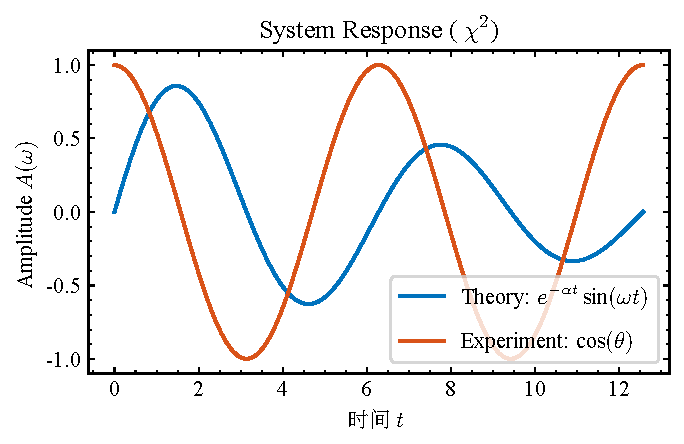
\includegraphics[width=\textwidth]{figures/example/example.pdf}
    \caption{实验组 A 结果}\label{fig:sub_a}
  \end{subfigure}
  \hfill % 弹性填充，将两图推向两侧
  % 第二张子图
  \begin{subfigure}[b]{0.45\textwidth}
    \centering
    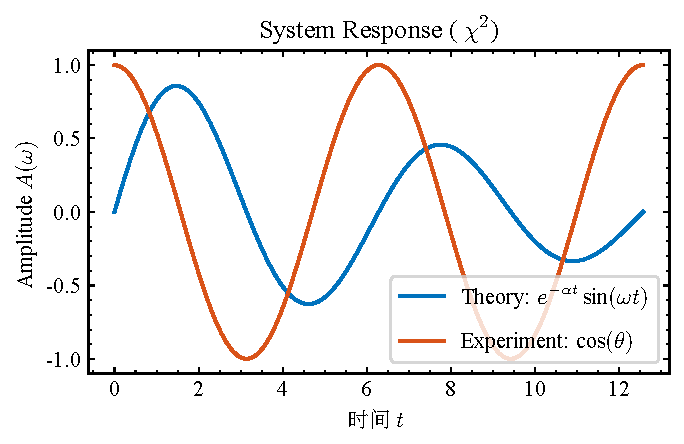
\includegraphics[width=\textwidth]{figures/example/example.pdf}
    \caption{对照组 B 结果}\label{fig:sub_b}
  \end{subfigure}
  \caption{不同实验条件下的结果对比（左：A组，右：B组）}\label{fig:comparison}
\end{figure}

如图~\ref{fig:comparison} 所示，我们成功实现了双图并排。且可以单独引用子图，例如图~\ref{fig:sub_a}。

\section{基于 tabularray 的专业表格}
相比传统表格环境，\texttt{tabularray} 宏包通过 \texttt{tblr} 环境提供了更简洁的语法。配合 \texttt{booktabs} 库，可以轻松绘制符合科技论文要求的“三线表”。

\begin{table}[htbp]
  \centering
  \caption{算法性能对比实验数据}\label{tab:example_data}
  \begin{tblr}{lrc}
    \toprule
    方法   & 准确率 (\%) & 耗时 (s) \\
    \midrule
    传统算法 & 85.2     & 0.45   \\
    神经网络 & 94.8     & 1.20   \\
    \bottomrule
  \end{tblr}
\end{table}

\section{自动化交叉引用}

引用数学公式： 式~\ref{eq:example_gauss}

引用图片： 图~\ref{fig:example_single}

引用表格： 表~\ref{tab:example_data}

引用文献： 文献~\cite{placeholder}  文献~\parencite{placeholder}
